\subsubsection{Analysis of a Simple Periodic Structure}
Expanding upon the simulation of a hemisphere, next, we analyse the deformation of a periodic structure that provides a comparison for the analysis of DNA imaging. As presented in Figure \ref{fig: Wave-ContourPlot}, the simulations produced 2D heat maps of the indention force across the cross-section of the surface. Comparison of cross sections for different indenter ratios, shown in Figure \ref{fig: Wave-ContourPlot-1} and Figure \ref{fig: Wave-ContourPlot-7}, shows that increasing indenter-to-surface ratios produces lower indentation forces. As with the hemisphere, due to the large contact radius, the forces are distributed over a large area; consequently, the compression is smaller for the same force. Moreover, evaluating the variation of the fitted Young's modulus over the scan positions, shown in Figure \ref{fig: Wave-Youngs},  highlights the relation between elastic response/ force and the contact area. Unlike for the hemisphere, the dependence on the tip-surface convolution produces an inverse relationship in Young's modulus at larger surface-tip ratios. At the surface trough, the indenter has a maximum contact radius and the maximum surface interaction. Consequently, the indenter experiences a larger effective stiffness and Young's modulus. However, the contact radius decreases for scans away from wave trough, and Young's modulus decreases proportionally.

\begin{figure}[ht]
\centering

    \begin{subfigure}[t]{0.325\textwidth}
        \centering
        \caption{\label{fig: Wave-ContourPlotNI-1} }
        \vspace{-0.1in}
             \begin{tikzpicture}
                \node (img1) {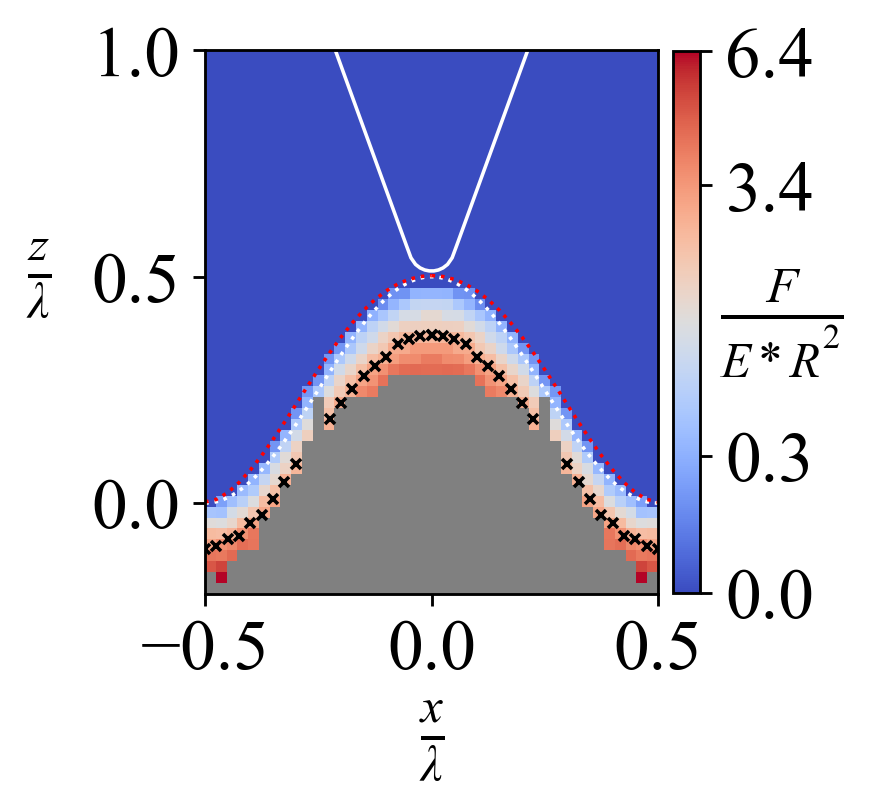
\includegraphics[trim = 57.5 60 58 10, clip, width=0.95\linewidth]{Figures/Wave-ContourPlotNI-1.png}};
                \node (img2) at ([xshift=1cm,yshift=-1cm]img1.north west) [scale=0.25] {\includegraphics[width=1\linewidth]{Figures/Axis.png}};
              \end{tikzpicture}
    \end{subfigure}
    \hfill
    \begin{subfigure}[t]{0.325\textwidth}
        \centering
        \caption{\label{fig: Wave-ContourPlotI-1} }
        \vspace{-0.1in}
             \begin{tikzpicture}
                \node (img1) {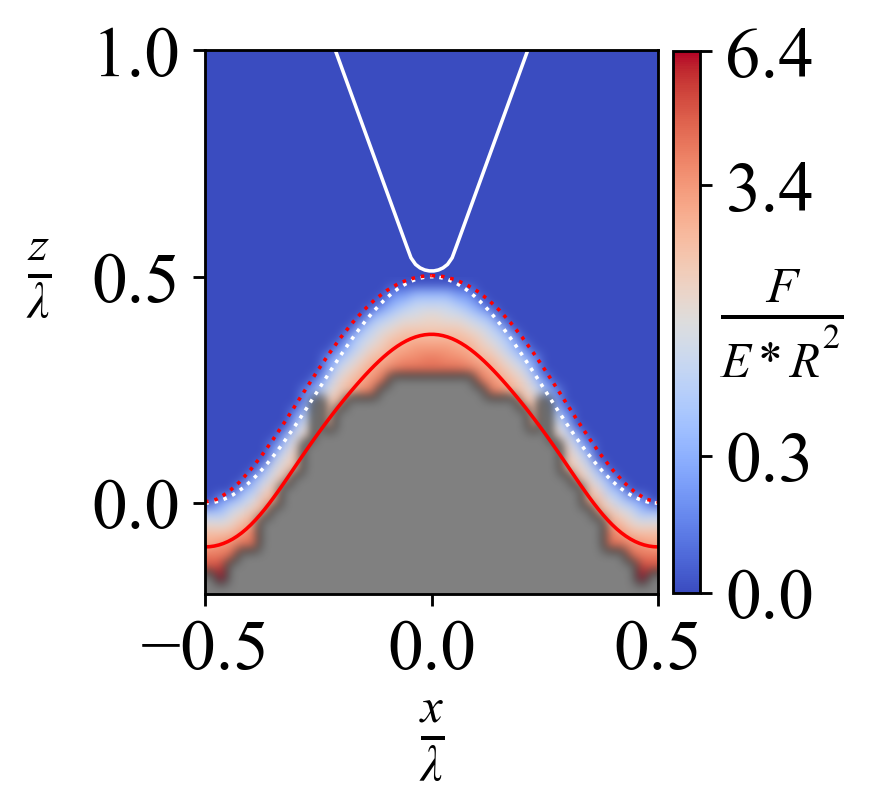
\includegraphics[trim = 57.5 60 58 10, clip, width=0.95\linewidth]{Figures/Wave-ContourPlot-1.png}};
                \node (img2) at ([xshift=1cm,yshift=-1cm]img1.north west) [scale=0.25] {\includegraphics[width=1\linewidth]{Figures/Axis.png}};
              \end{tikzpicture}
    \end{subfigure}
    \hfill
    \begin{subfigure}[t]{0.325\textwidth}
        \centering
        \caption{\label{fig: Wave-LineContour-1} }
        \vspace{-0.1in}
             \begin{tikzpicture}
                \node (img1) {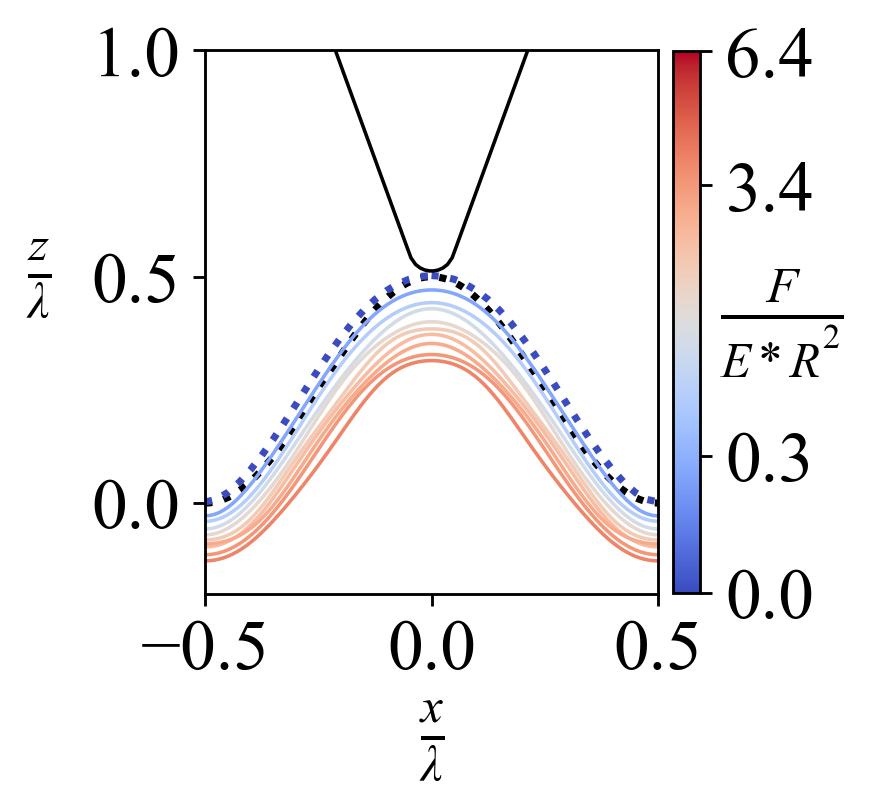
\includegraphics[trim = 57.5 60 58 10, clip, width=0.95\linewidth]{Figures/Wave-LineContour-1.png}};
                \node (img2) at ([xshift=1cm,yshift=-1cm]img1.north west) [scale=0.25] {\includegraphics[width=1\linewidth]{Figures/Axis.png}};
              \end{tikzpicture}
    \end{subfigure} 
    
    \caption{\label{fig: Wave-ContourPlot}Illustrations of data produced from compression simulations for indenter $R/\lambda=0.05$. (A) Raw two-dimensional heat map of indentation force over the scanning axis for the periodic structure. Including the point of constant force, $\frac{F}{E^*R^2} = 0.227 $, shown as black crosses. These are points used to produce the force contours. The indenter is solid white, and the surface is dotted white. Points of zero force/ hard sphere contact is shown in dotted red.(B) Interpolated two-dimensional heat map of indentation force over the scanning axis for the periodic structure. Including overlayed contour of constant force, $\frac{F}{E^*R^2} = 0.227 $, shown in solid red. The indenter is solid white, and the surface is dotted white. Points of zero force/ hard sphere contact is shown in dotted red. (C) Two-dimensional plot of force contours for varying indentation/ reference forces over the scanning axis of the periodic structure. Force shown varies within the limit of $ 0.227 < \frac{F}{E^*R^2} < 3.867 $. The indenter and surface are black with initial zero force/ hard sphere boundary in dashed blue.}
    
\end{figure}

For greater quantitative analysis of the compression in the simulation, both Fourier analysis and FWHM are employed. Fitting the contour points using a Fourier series allows us to break down the oscillatory signature of the simulated surface appearance. Furthermore, the individual contribution can highlight the deviation and behaviour of the surface when indented. The Fourier components are shown in Figure \ref{fig: Wave-Fourier}. The zeroth component of the Fourier series represents a linear vertical offset. The increasing trend corresponds to an increased trough height for larger indenter-surface ratios. The first component corresponds to surface periodicity. Only this component is expected for the contour that matches the geometry of the surface, as shown by the black bar in Figure \ref{fig: Wave-Fourier}. The decreasing amplitude of this component corresponds to an increase in surface distortion, as the amplitude is shared proportionally with higher-order terms. The second component is the significant component producing the widening wave peak, and higher-order terms refine the curvature of the contour. 

\begin{figure}[H]
\centering

    \begin{subfigure}[t]{0.3\textwidth}
        \centering
        \caption{\label{fig: Wave-Setup} }
        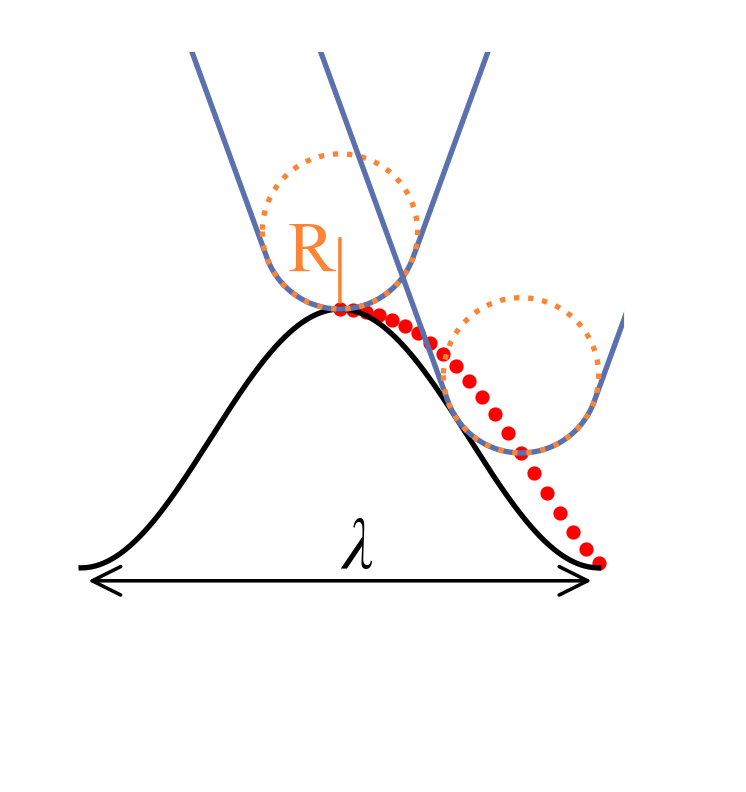
\includegraphics[width=1\linewidth]{Figures/Wave-SetUp.png}
    \end{subfigure}
    \hfill
    \begin{subfigure}[t]{0.34\textwidth}
        \centering
        \caption{\label{fig: Wave-ContourPlot-1} }
        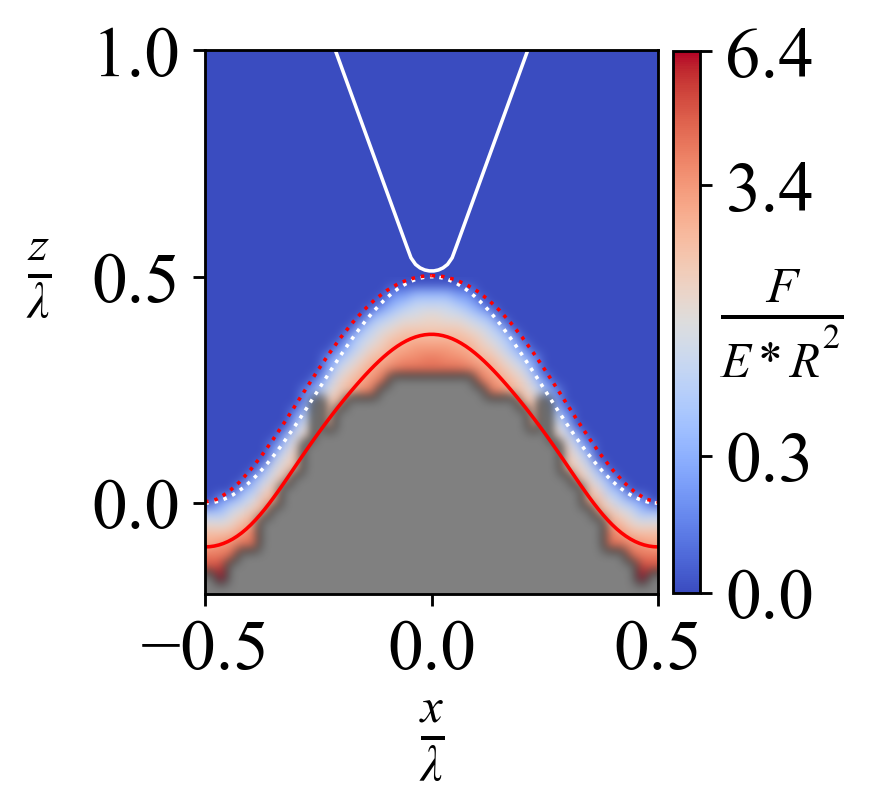
\includegraphics[width=1\linewidth]{Figures/Wave-ContourPlot-1.png}
    \end{subfigure}
    \hfill
    \begin{subfigure}[t]{0.34\textwidth}
        \centering
        \caption{\label{fig: Wave-ContourPlot-7} }
        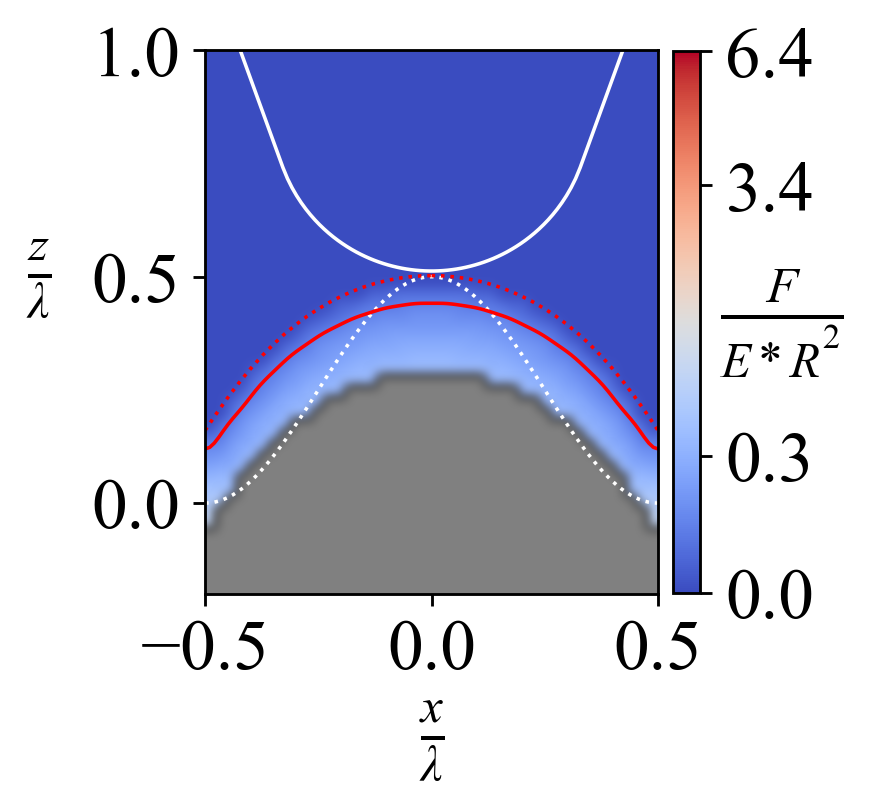
\includegraphics[width=1\linewidth]{Figures/Wave-ContourPlot-7.png}
    \end{subfigure}

    
     \hfill
    \vspace{-0.3in}

    \begin{subfigure}[t]{0.325\textwidth}
        \centering
        \caption{\label{fig: Wave-Youngs} }
        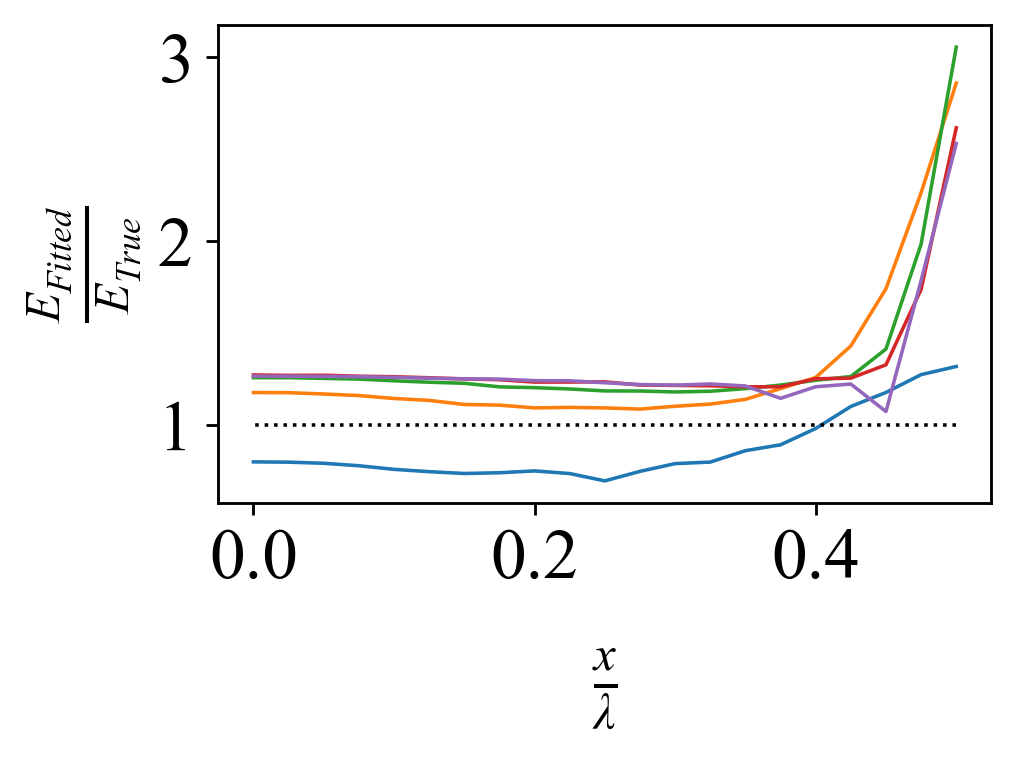
\includegraphics[width=1\linewidth]{Figures/Wave-Youngs.png}
    \end{subfigure}
     \hfill
    \begin{subfigure}[t]{0.325\textwidth}
        \centering
        \caption{\label{fig: Wave-FWHM} }
        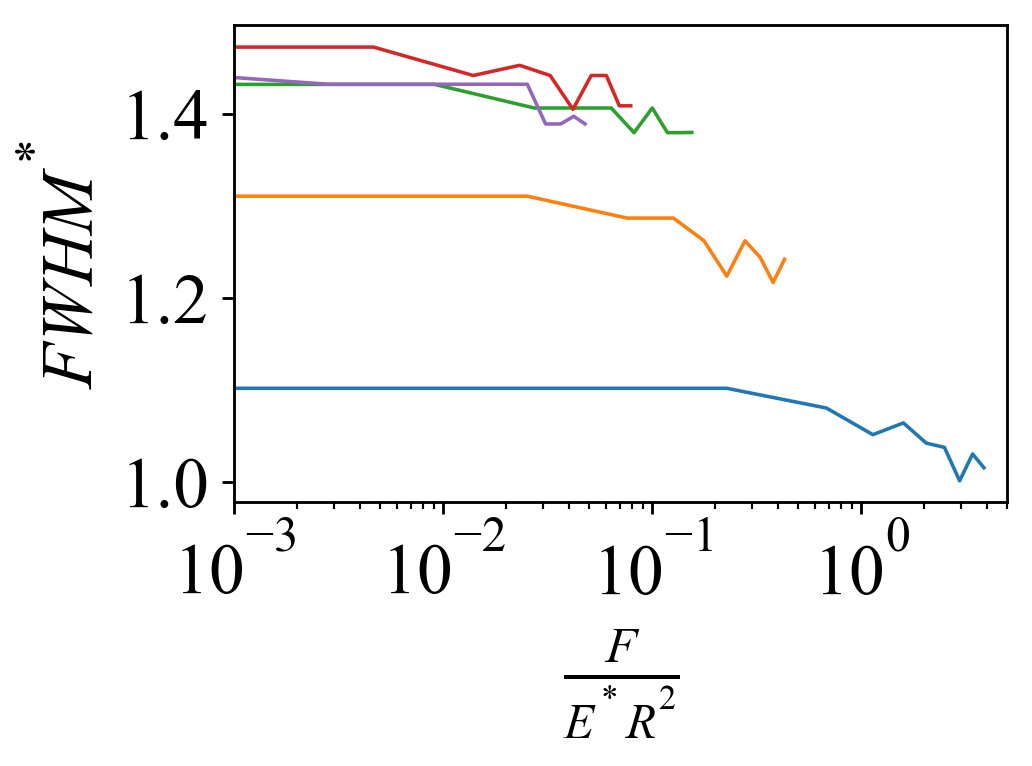
\includegraphics[width=1\linewidth]{Figures/Wave-FWHM.png}
    \end{subfigure}    
     \hfill
    \begin{subfigure}[t]{0.325\textwidth}
        \centering
        \caption{\label{fig: Wave-Volume} }
        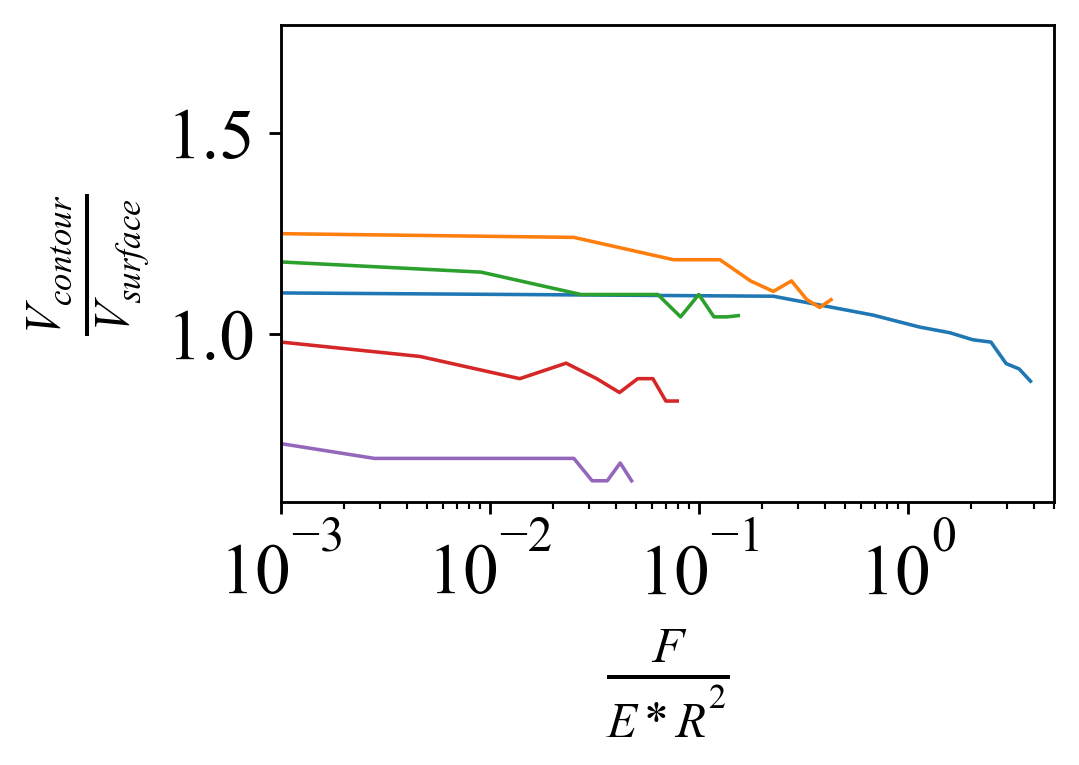
\includegraphics[width=1\linewidth]{Figures/Wave-Volume.png}
    \end{subfigure}

     \hfill
     
    \begin{subfigure}[t]{1\textwidth}
        \centering
        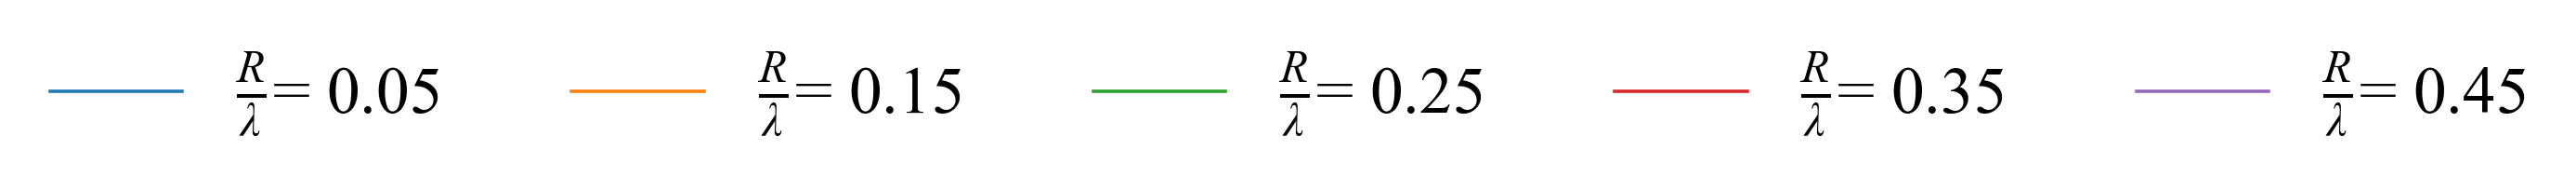
\includegraphics[width=1\linewidth]{Figures/Wave-Legend.png}
    \end{subfigure}

    \caption{\label{fig: Wave Compression Plot}(A) Geometry of scan along the central axis of a hemisphere. Three-dimensional geometry is produced by rotating the indenter and extruding the wave. Wave is shown in black with wavelength $\lambda$. Indenter geometry is shown in blue with a circular tip of radius $R$ in orange. Red points indicate initial scan positions (Hard sphere contact points). (B) Interpolated two-dimensional heat map of indentation force over the scanning axis for periodic structure with indenter $R/\lambda=0.05$. Including overlayed contour of constant force, $\frac{F}{E^*R^2} = 0.227 $, shown in solid red. The indenter is solid white, and the surface is dotted white. Points of zero force/ hard sphere contact is shown in dotted red. (C) Interpolated two-dimensional heat map of indentation force over the scanning axis for periodic structure with indenter $R/\lambda=0.45$. Including overlayed contour of constant force, $\frac{F}{E^*R^2} = 0.227 $, shown in solid red. The indenter is solid white, and the surface is dotted white. Points of zero force/ hard sphere contact is shown in dotted red. (D) Fitted Young's modulus over scan positions for each indenter radius ($R/\lambda$). (E) Relative FWHM of the contour divided by FWHM of true geometry ($FWHM^*=\frac{FWHM}{FWHM_{True}}$) variation over contour force for each indenter radius($R/\lambda$). (F)  Volume variation over contour force in spherical structures for each indenter radius($R/\lambda$).}
    
\end{figure}


Therefore, the deviation from the true surface geometry and accuracy of the imaging can be quantified by analysing the variation of the first Fourier component over a range of contour forces. Analysing the absolute A1 for each contour force, shown in \ref{fig: Wave-Fourier True Component}, indicates how well we extract information from the surface topography. A lower indenter-surface ratio produces less apparent structure deviation as the scan/tip more closely follows the surface geometry. Moreover, A1 is generally constant over the range of contour forces with only some decrease in the component for the smaller indenter at larger forces.  

However, in contrast, the relative component $A^*_1$ (i.e. individually normalised series where $A_1+A_2+A_3+... = 1$) shows that although the absolute value of the first component may be constant throughout the forces range, the actual percentage of the series that the first component represents does vary. As shown in Figure \ref{fig: Wave-Fourier Relative Component}, when contour force increases, a greater percentage of the periodicity of the surface is recovered. This indicates that the apparent resolution extracted from the AFM image increases with indentation force. This could be due to the increased proportion of the indenter in contact with the surface and the elastic behaviour becoming more linear for deeper  indentations. As a result, the indentations are subject to more influence from the surfaces. Therefore, variations in the surface geometry are better resolved in the contour at a higher force. 

\begin{figure}[ht]
\centering

    \begin{subfigure}[t]{1\textwidth}
        \centering
        \caption{\label{fig: Wave-Fourier}}
        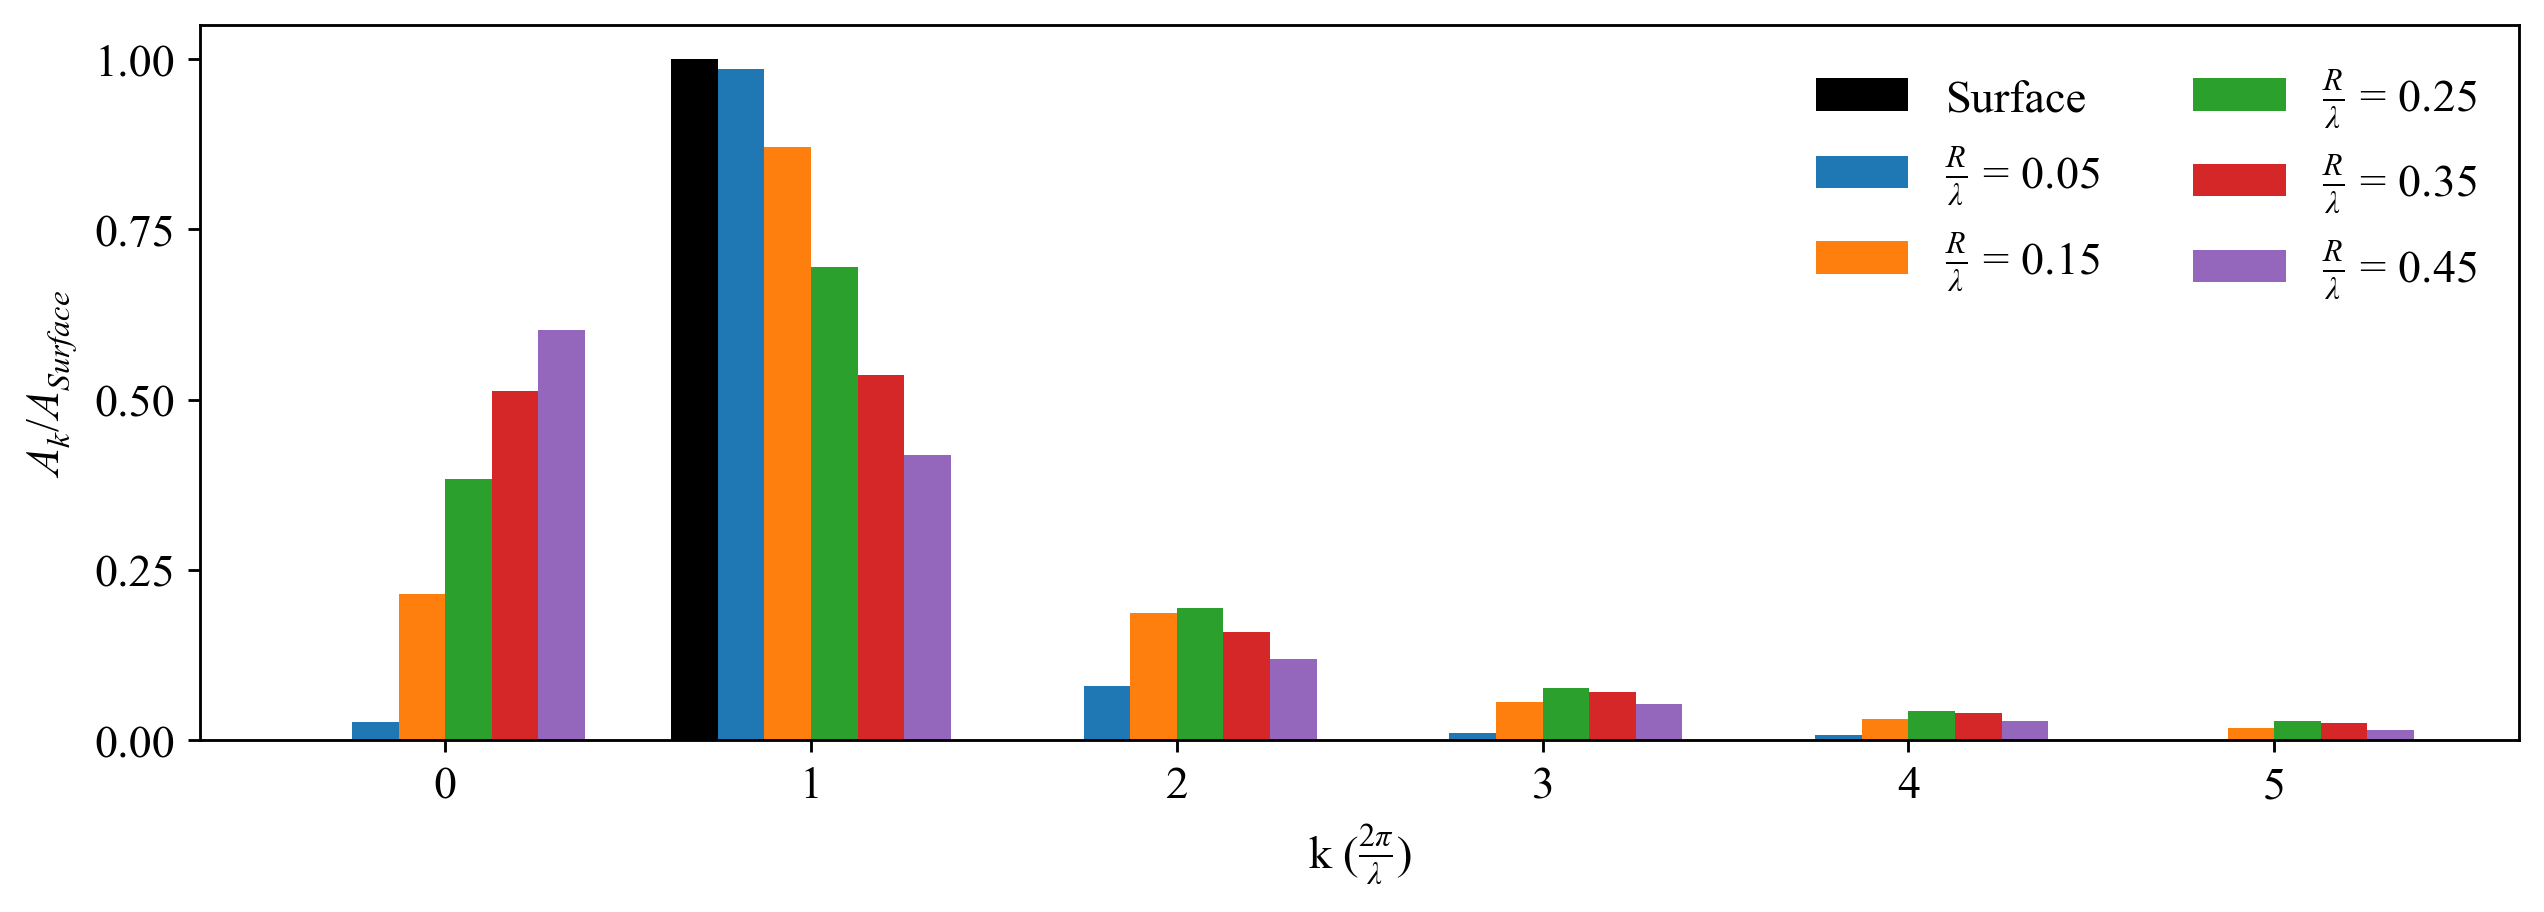
\includegraphics[width=1\linewidth]{Figures/Wave-Fourier1.png}
    \end{subfigure}
    
    \hfill
    
    \begin{subfigure}[t]{0.325\textwidth}
        \centering
        \caption{\label{fig: Wave-Fourier True Component} }
        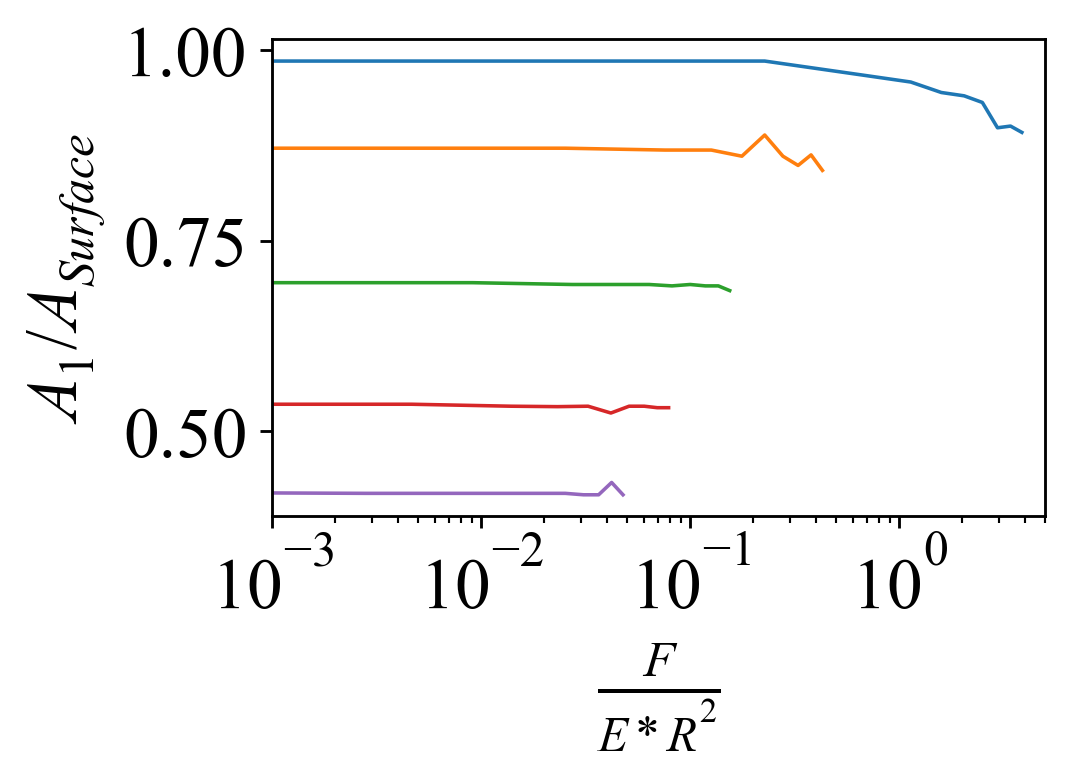
\includegraphics[width=1\linewidth]{Figures/Wave-Fourier4.png}
    \end{subfigure}    
    \hfill    
    \begin{subfigure}[t]{0.325\textwidth}
        \centering
        \caption{\label{fig: Wave-Fourier Relative Component} }
        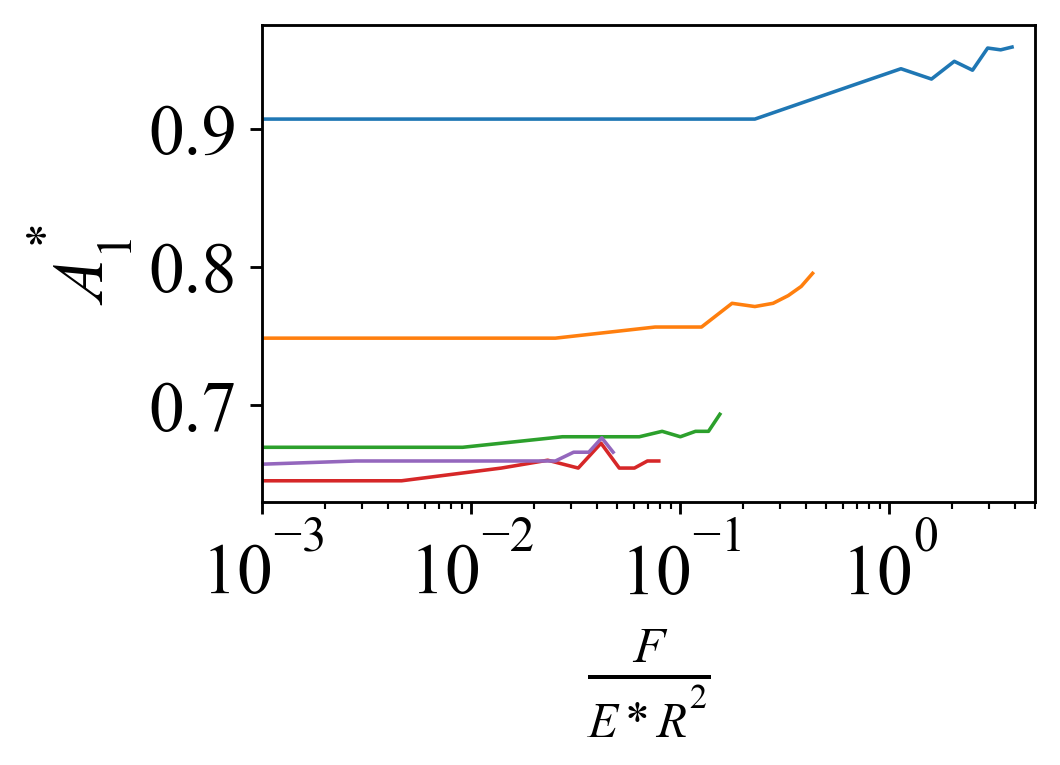
\includegraphics[width=1\linewidth]{Figures/Wave-Fourier3.png}
    \end{subfigure}
    \hfill
    \begin{subfigure}[t]{0.325\textwidth}
        \centering
        \caption{\label{fig: Wave-FWHM-Fourier} }
        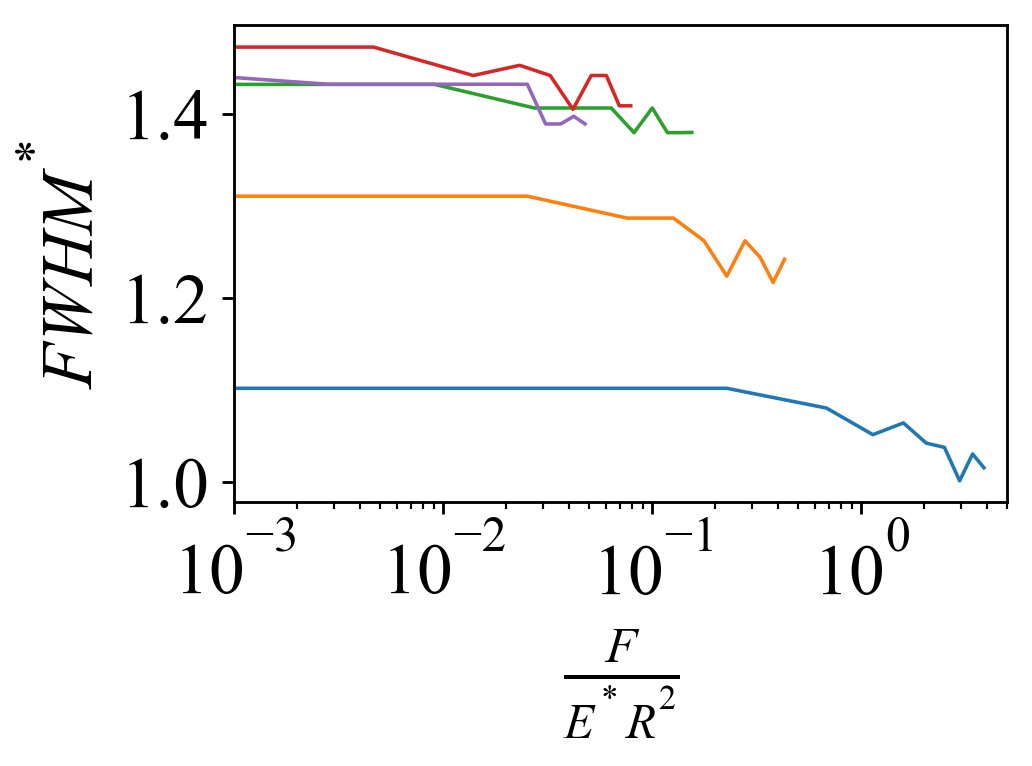
\includegraphics[width=1\linewidth]{Figures/Wave-FWHM.png}
    \end{subfigure}    

    \hfill
    
    \begin{subfigure}[t]{1\textwidth}
        \centering
        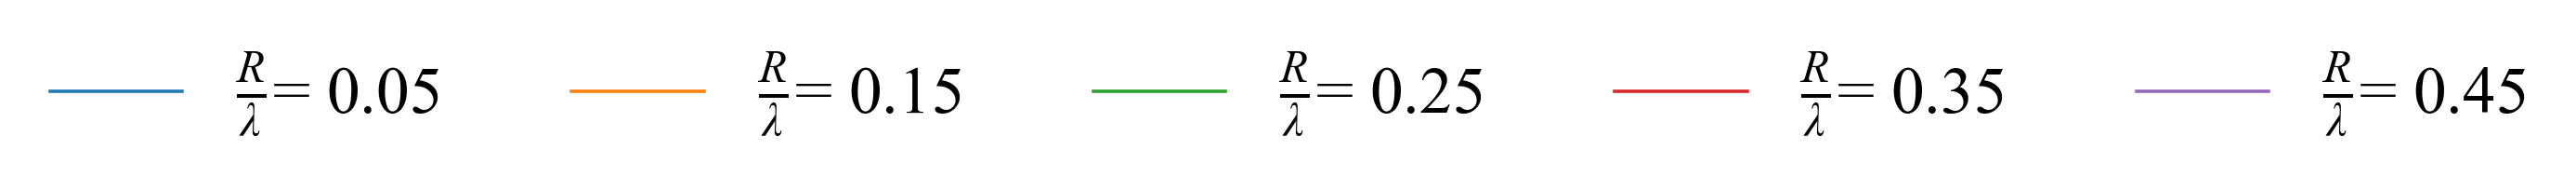
\includegraphics[width=1\linewidth]{Figures/Wave-Legend.png}
    \end{subfigure}

    
    \caption{\label{fig: Wave FWHM/Fourier}Analysis of force contours for periodic structure. (A) Fourier Series Component for force contours at $\frac{F}{E*R^2} = 0.227$. (B) Variation of absolute component $A_1$ (Normalised by true surface amplitude/Fourier component) over contour force for a range of indenters ($\frac{R}{\lambda}$). (C) Variation of relative component $A_1^*$ ($A_1$ coeffiecent normalised by series terms - $A_1^*=\sum_{k\neq0}A_k$) over contour force for range of indenters ($\frac{R}{\lambda}$). (D) Relative FWHM of the contour divided by FWHM of true geometry ($FWHM^*=\frac{FWHM}{FWHM_{Surface}}$) variation over contour force for each indenter radius($\frac{R}{\lambda}$).}
    
\end{figure}

This behaviour is supported by the FWHM shown in Figure \ref{fig: Hemisphere FWHM}. As the indentation force increases, FWHM decreases asymptotically, similarly to the absolute component $A1$, which represents the compression of the sample. This produces contours with FWHM closer to the true FWHM. Comparing this with the trends highlighted in Fourier analysis further reinforces that larger forces enable better resolution of the underlying structure. The initial constant trend of the FWHM may also show that at low forces, the compression around the midpoint of the wave is low, and the indenter requires a large force to indent the slope region.

As shown in Figure \ref{fig: Hemisphere-Volume}, the volume variation over indentation force is less prominent than for the hemisphere. For each indenter, there is only a slight reduction in volume as the indentation force increases. Moreover, unlike the hemisphere, the apparent volume is not directly proportional to the indenter's radius. Although a larger indenter produces greater tip convolution, which widens the peak, as volume is measured from the peak to the trough, the composite reduction in wave amplitude and depth results in a smaller volume overall as the indenter radius increases from $R/\lambda =0.15$. In contrast, $R/\lambda =0.15$ produces force contours closer to the topology of the surfaces, which is reflected in the apparent volume. 

Overall, these analyses highlight similar characteristics to the hemisphere under compression. Young's modulus shows the dependence of elastic response/behaviour on the contact radius and tip convolution. Similarly, the volume highlights that the larger indenters/contact areas require larger forces to compress the sample to the same extent as smaller indenters. However, the FWHM and Fourier analysis elucidate a possible novel feature. The Fourier analysis demonstrates that larger indentation forces recover more surface periodicity.